%%
%% This is file `mcmthesis-demo.tex',
%% generated with the docstrip utility.
%%
%% The original source files were:
%%
%% mcmthesis.dtx  (with options: `demo')
%% 
%% -----------------------------------
%% 
%% This is a generated file.
%% 
%% Copyright (C)
%%       2010 -- 2015 by Zhaoli Wang
%%       2014 -- 2019 by Liam Huang
%%       2019 -- present by latexstudio.net
%% 
%% This work may be distributed and/or modified under the
%% conditions of the LaTeX Project Public License, either version 1.3
%% of this license or (at your option) any later version.
%% The latest version of this license is in
%%   http://www.latex-project.org/lppl.txt
%% and version 1.3 or later is part of all distributions of LaTeX
%% version 2005/12/01 or later.
%% 
%% This work has the LPPL maintenance status `maintained'.
%% 
%% The Current Maintainer of this work is latexstudio.net.
%% 
%%
%% This is file `mcmthesis-demo.tex',
%% generated with the docstrip utility.
%%
%% The original source files were:
%%
%% mcmthesis.dtx  (with options: `demo')
%%
%% -----------------------------------
%%
%% This is a generated file.
%%
%% Copyright (C)
%%       2010 -- 2015 by Zhaoli Wang
%%       2014 -- 2019 by Liam Huang
%%       2019 -- present by latexstudio.net
%%
%% This work may be distributed and/or modified under the
%% conditions of the LaTeX Project Public License, either version 1.3
%% of this license or (at your option) any later version.
%% The latest version of this license is in
%%   http://www.latex-project.org/lppl.txt
%% and version 1.3 or later is part of all distributions of LaTeX
%% version 2005/12/01 or later.
%%
%% This work has the LPPL maintenance status `maintained'.
%%
%% The Current Maintainer of this work is Liam Huang.
%%
\documentclass{mcmthesis}
\mcmsetup{CTeX = false,   % 使用 CTeX 套装时,设置为 true
        tcn = 2100079, problem = B,
        sheet = true, titleinsheet = true, keywordsinsheet = true,
        titlepage = true, abstract = true}
\usepackage{newtxtext}%\usepackage{palatino}
\usepackage{lipsum}
\title{Our Thesis for 2021 MCM Problem B}
%\author{Muyuan Peng \quad Wei Zhao \quad Zhenyu Zhao}
\date{\today}
\begin{document}
\begin{abstract}
 

\begin{keywords}
keyword1; keyword2
\end{keywords}
\end{abstract}
\maketitle
%% Generate the Table of Contents, if it's needed.
%% \tableofcontents
%% \newpage
%%
%% Generate the Memorandum, if it's needed.
%% \memoto{\LaTeX{}studio}
%% \memofrom{Liam Huang}
%% \memosubject{Happy \TeX{}ing!}
%% \memodate{\today}
%% \logo{\LARGE I'm pretending to be a LOGO!}
%% \begin{memo}[Memorandum]
%%   \lipsum[1-3]
%% \end{memo}
%%
\tableofcontents
\newpage
\section{Overview}
\subsection{Background}


 The wildfires in Australia recently has drawn great focus. Frequent wildfires bring fire extinguishing system great pressure, thus the assistance
of automatic devices, like Unmanned Aerial Vehicle(UAV), 
radio and unmanned reconnaissance, should be taken into considerition. 
\subsection{Restatement of the Problem}

To help the firefighting system in East Victoria State, we are required
to solve several problems. The unmanned devices to respond to the bushfires can be divided to two kinds,
the SSA Thermal Imaging system and the Radio Repaeters, with each UAV carrying
one of them. To gurantee that the Safty Cofficient meets the satandard, we should
balance the number of SSA and RR carried by UAVs, in order to acquire best economic benifits.\\
Moreover, the prediction of the bushfires in the next decade in East Victotia is required
we will explain how to apply our model to respond to the bushfires.We are also required 
to point out where the UAVs with Radio Repaeters should be.

\begin{figure}[htbp]
  \centering
  \includegraphics[scale=0.7]{figures/Vict_Map.png}
  \caption{Topographical Map of Eastern Victoria}
  \label{Topographical Map of Eastern Victoria}
\end{figure}


\section{Notations}
\begin{itemize}
  \item \textbf{Unmanned Aerial Vehicle} $\rightarrow$ UAV
  \item \textbf{Radio Repeater} $\rightarrow$ RR
  \item \textbf{Rapid Bushfire Response} $\rightarrow$ RBR
  \item \textbf{Surveillance and Situational Awareness} $\rightarrow$ SSA
  \item \textbf{The total number of SSA and RR}$\rightarrow$ M
  \item \textbf{The number of firespot}$\rightarrow$ x
  \item \textbf{The number of fireregion}$\rightarrow$ y
  \item \textbf{The number of firefighters}$\rightarrow$ F
  \item \textbf{Vector (x,y)}$\rightarrow$ $\alpha$ 
  \item \textbf{Danger Cofficient}$\rightarrow$ d
\end{itemize}
\newpage


\section{Hypothesis and Justifications}
\begin{enumerate}
  \item \textbf{The EOC will be set near the fire and will not move}
  \item \textbf{The Radio Repaeters'(RR) flights are always at their highest speed and will keep their location at the fires}
  \item \textbf{The wildfires are considered as discrete dots(Firepoints)} 
  \item \textbf{The UAV with SSA system must work within 5Km from the firepoint}
  \item \textbf{Ignore the side effects like Doppler Effecet and the influence of the winds}
\end{enumerate}

\section{Model Overview}
\subsection{Model Notations}
\begin{itemize}
  \item $M_1$: number of SSA
  \item $M_2$: number of RR
  \item $M=M_1+M_2$: number of drones
\end{itemize}

\subsection{Model Assumptions and Justifications}
\begin{itemize}
  \item Firefireghters number F=50
  \item The locations of RR should gurantee that all targets(firefighters and firepoints)
  in a radius of 5Km, and stay still
  \item Due to the limit of battery the drones won't take a long flight. We assume
  that the fire map is not big to gurantee that each RR can communicate directly with EOC
  \item After the gurantee of RR, we only need to consider the economic benefits of SSA
\end{itemize}
\subsection{Model 1: Optimal numbers Model}
To design a purchasing configuration for SSA and RR, we need to introduce a \textbf{Danger Cofficient}
to evaluate whether the number of devices can gurantee that the firefightres are safe enough to work at
the firespots. Due to various kinds of goods in the problem, this is a threedimensional
heterogeneous container loading problem. We use the Three Space Division
Method and Monte Carlo Simulation to solve it.

\subsubsection{{SubModel 1: Fire Map}}
To describe the distribution of firespots, fireregions and thus the location
of firefighters. We produce random location of fireregions and firespots, and thus
the locations of firefighters. Therefor, a firemap is produced. 
\begin{figure}[htbp]
  \centering
  \includegraphics[scale=0.7]{figures/Str_1.png}
  \caption{Overview of Firemap}
  \label{Overview of Firemap}
\end{figure}




\subsubsection{SubModel 2: Drones Distribution}
Once a firemap is produced, each distribution of $M_1 and M_2$ will has a so-called
\textbf{Danger Cofficient $d$} corresponding to it. Obviously, with \textbf{M} increasing, 
\textbf{d} will reduces.\\
In order to get better economic benefits, we should take the cost on the drones
into considerition. Once we get the minimum of cost, the project is considered to be optimal. 

\subsection{Model 2: The adaptation to the changing fire conditions}
According to previous fire conditions measured by the satellites, in other words, 
the abnormal spots every day and with the various topographical structure, we can cluster the abnormal spots to firespots through
\textbf{Cluster Analysis} and moreover we can obtain fireregions. Thus we can \textbf{predict
and arrange} the number of SSA and RR on drones, even \textbf{in the next decade}.
\vspace{5pt}
\begin{figure}[htbp]
  \centering
  \includegraphics[scale=0.53]{figures/Str_2.png}
  \caption{Optimal Number}
  \label{Optimal Number}
\end{figure}









\section{Model Theory}
\subsection{Optimal Drones Model}
\begin{itemize}
  \item \textbf{First}, we'd like to set fires at differnt locations in Eastern Victoria, called firespots 
  and fireregions. In certain radius, we set 2 or 3 fireregions with several random firespots
  in the fireregions. But the range of \textbf{y} ($R_y$)is correlated with number of \textbf{x}.
\begin{equation}
  R_y=y^{0.3}
\end{equation}
  \item \textbf{Second}, we introduce \textbf{d} for firespots and firefighters. If F or x are not in the sight of 
  Thermal Camera on SSA, \textbf{d} will increases with time going on. Once \textbf{F} or \textbf{x} are spotted by SSA,
  \textbf{$d_F$ and $d_x$} will vanish.
  \begin{equation}
    d_F=C_1t^2
  \end{equation}
  \begin{equation}
    d_x=C_2t  
  \end{equation}
  \item \textbf{Third}, according to the flights of the drones, we will colletct \textbf{$d_F$ and $d_x$}
  every 15 seconds. According to means of \textbf{$d_F$ and $d_x$} and the economic effects, we can decide the number
  of differnt kinds of drones. Totally we will colletct 480 series of data, and the sum
  of the 480 D is considered as the final Danger Cofficient.
  \begin{equation}
    D=Means \quad of \quad  d_F+ Means\quad  of\quad  d_x
  \end{equation}
  \item If the total cost function W reach the minimum when d meets the standard, we think that it is the best project.
  \begin{equation}
    W=k_1M+k_2d
  \end{equation}
  \item To subtitude the drones running out of fussel, we need subtitution drones
  always on their way to subtitution, and we need to calculate the number of subtitution drones.
 \begin{itemize}
   \item Cost of electricity still is $a=1/150Km^{-1}$, and the cost at flight
   is $b=1/25Km^{-1}$
   \item The speed of flight is $v=1.2Km/Min$
 \end{itemize}
 As a Result, the number of RR required at the distance of k from base, the
\end{itemize}
\begin{figure}[htbp]
  \centering
  \includegraphics[scale=0.7]{figures/Str_3.png}
  \caption{Optimal Number}
  \label{Optimal Number}
\end{figure}
\newpage

\section{Model Implementation and Results}
\subsection{Imgaes}
According to our method to make a firemap, we produce a simulated map as below:

\begin{figure}[htbp]
  \centering
  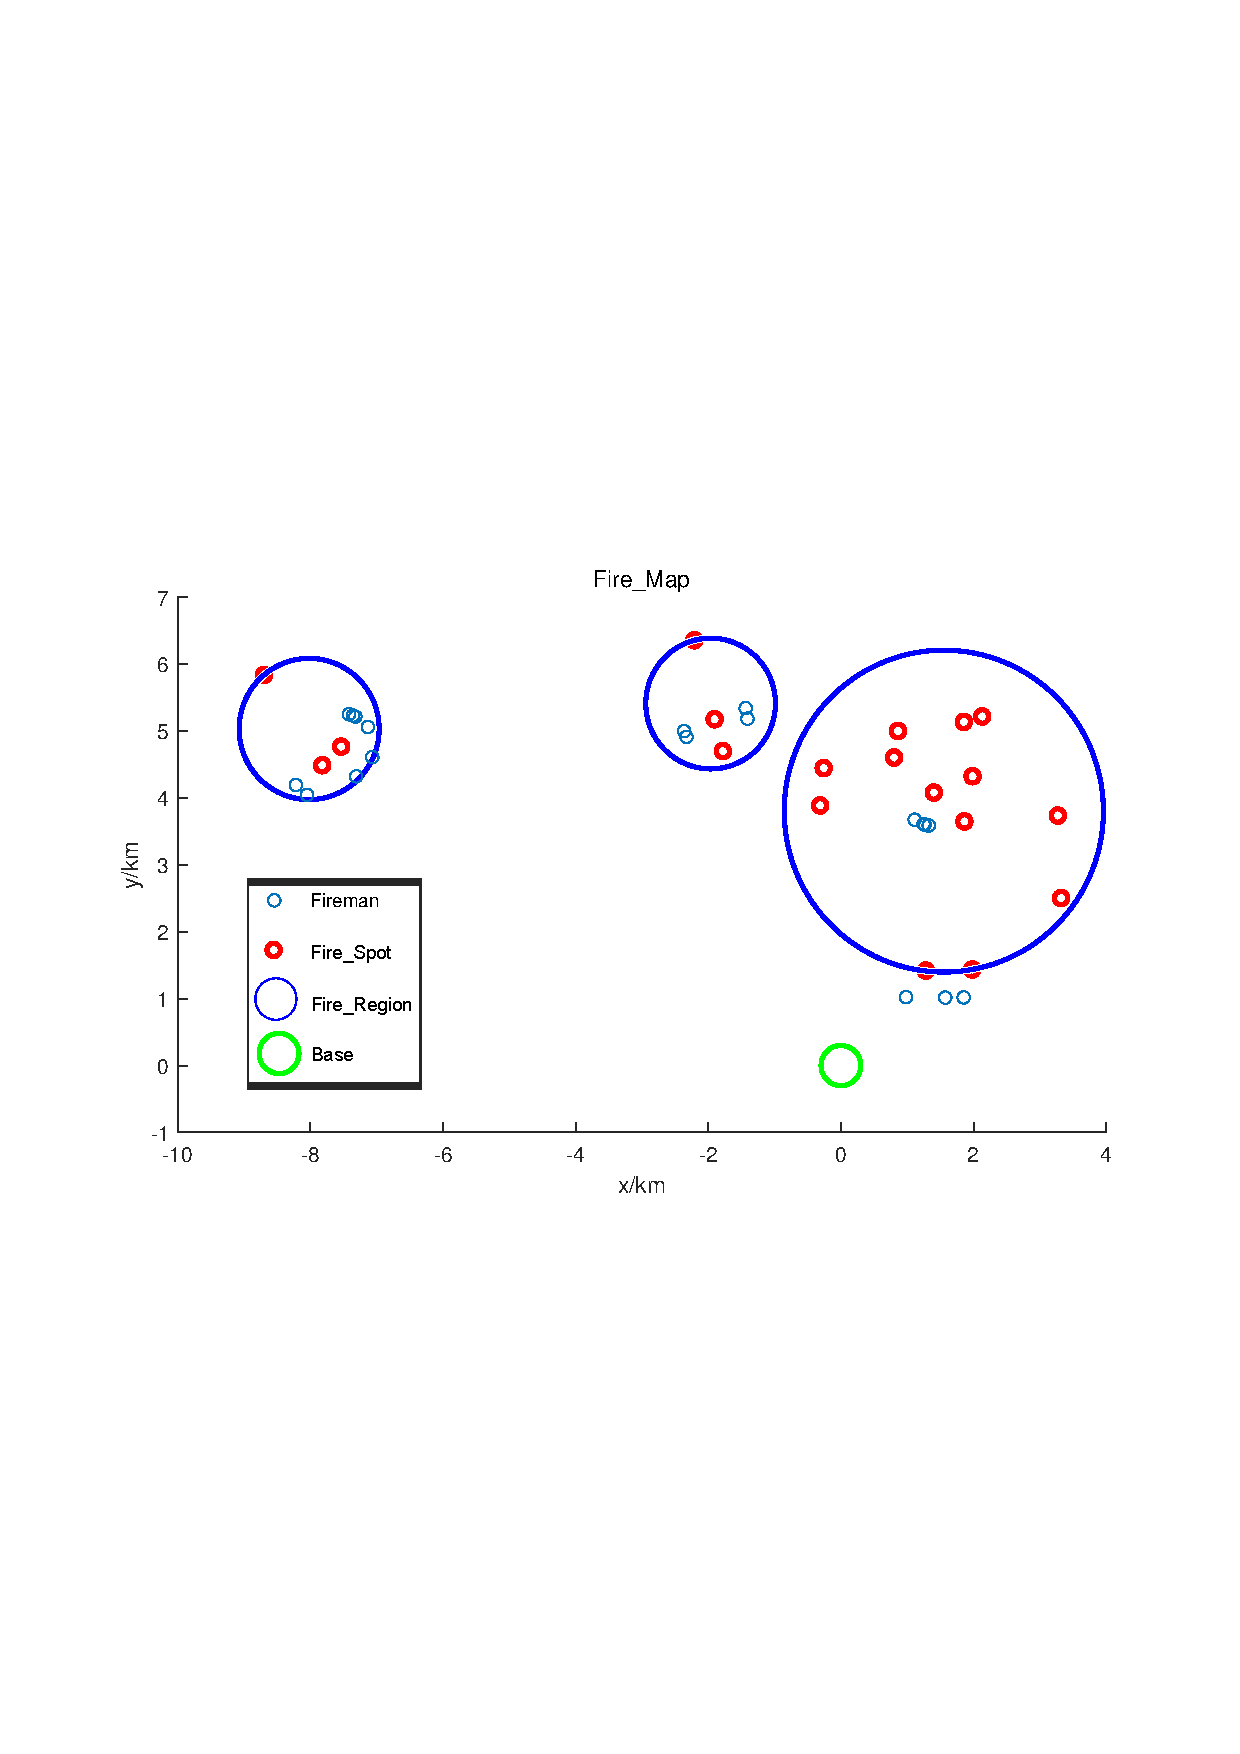
\includegraphics[scale=0.7]{figures/Fire_Map_demo.pdf}
  \caption{Firemap}
  \label{Firemap}
\end{figure}

\begin{figure}[htbp]
  \centering
  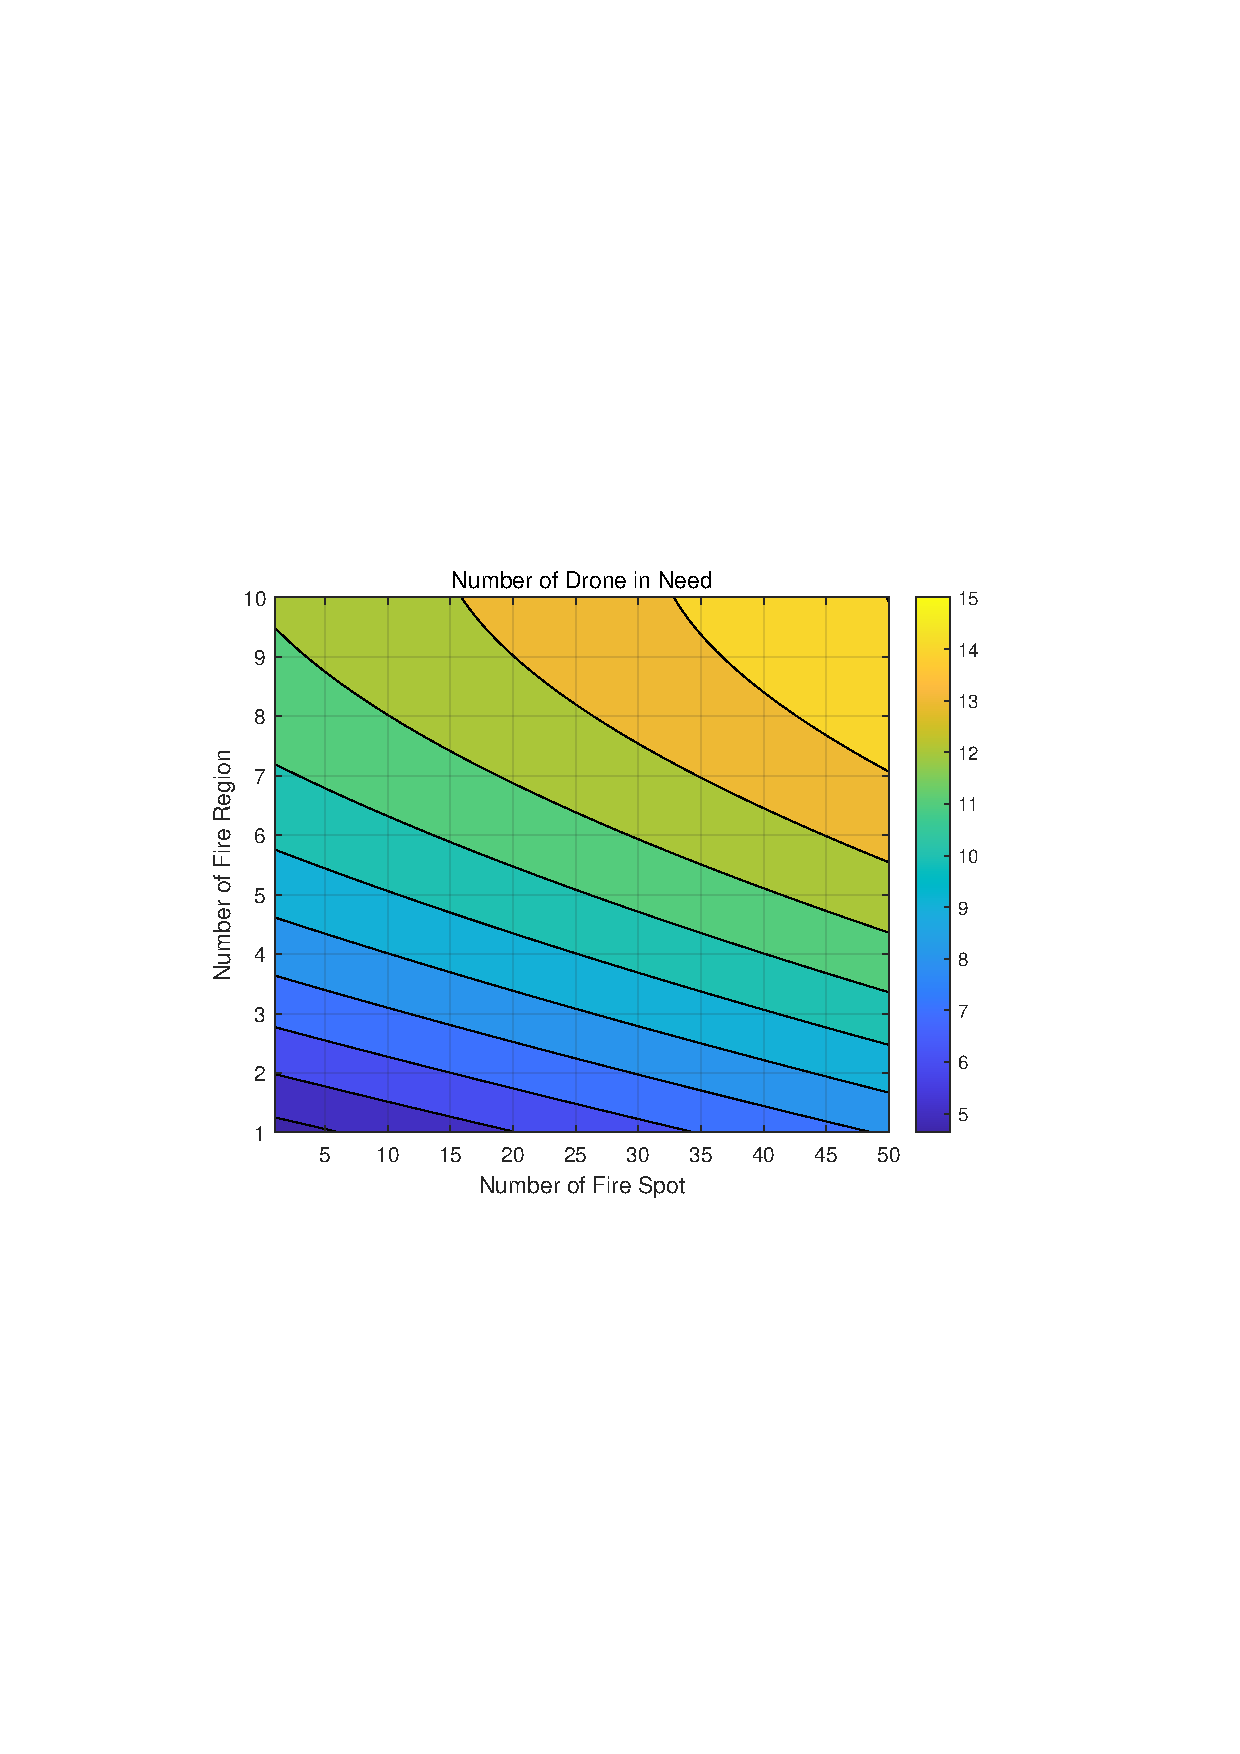
\includegraphics[scale=0.5]{figures/Number_of_Drone_in_Need_contour.png}
  \caption{Drone Number}
  \label{Drone Number}
\end{figure}

\begin{figure}[htbp]
  \centering
  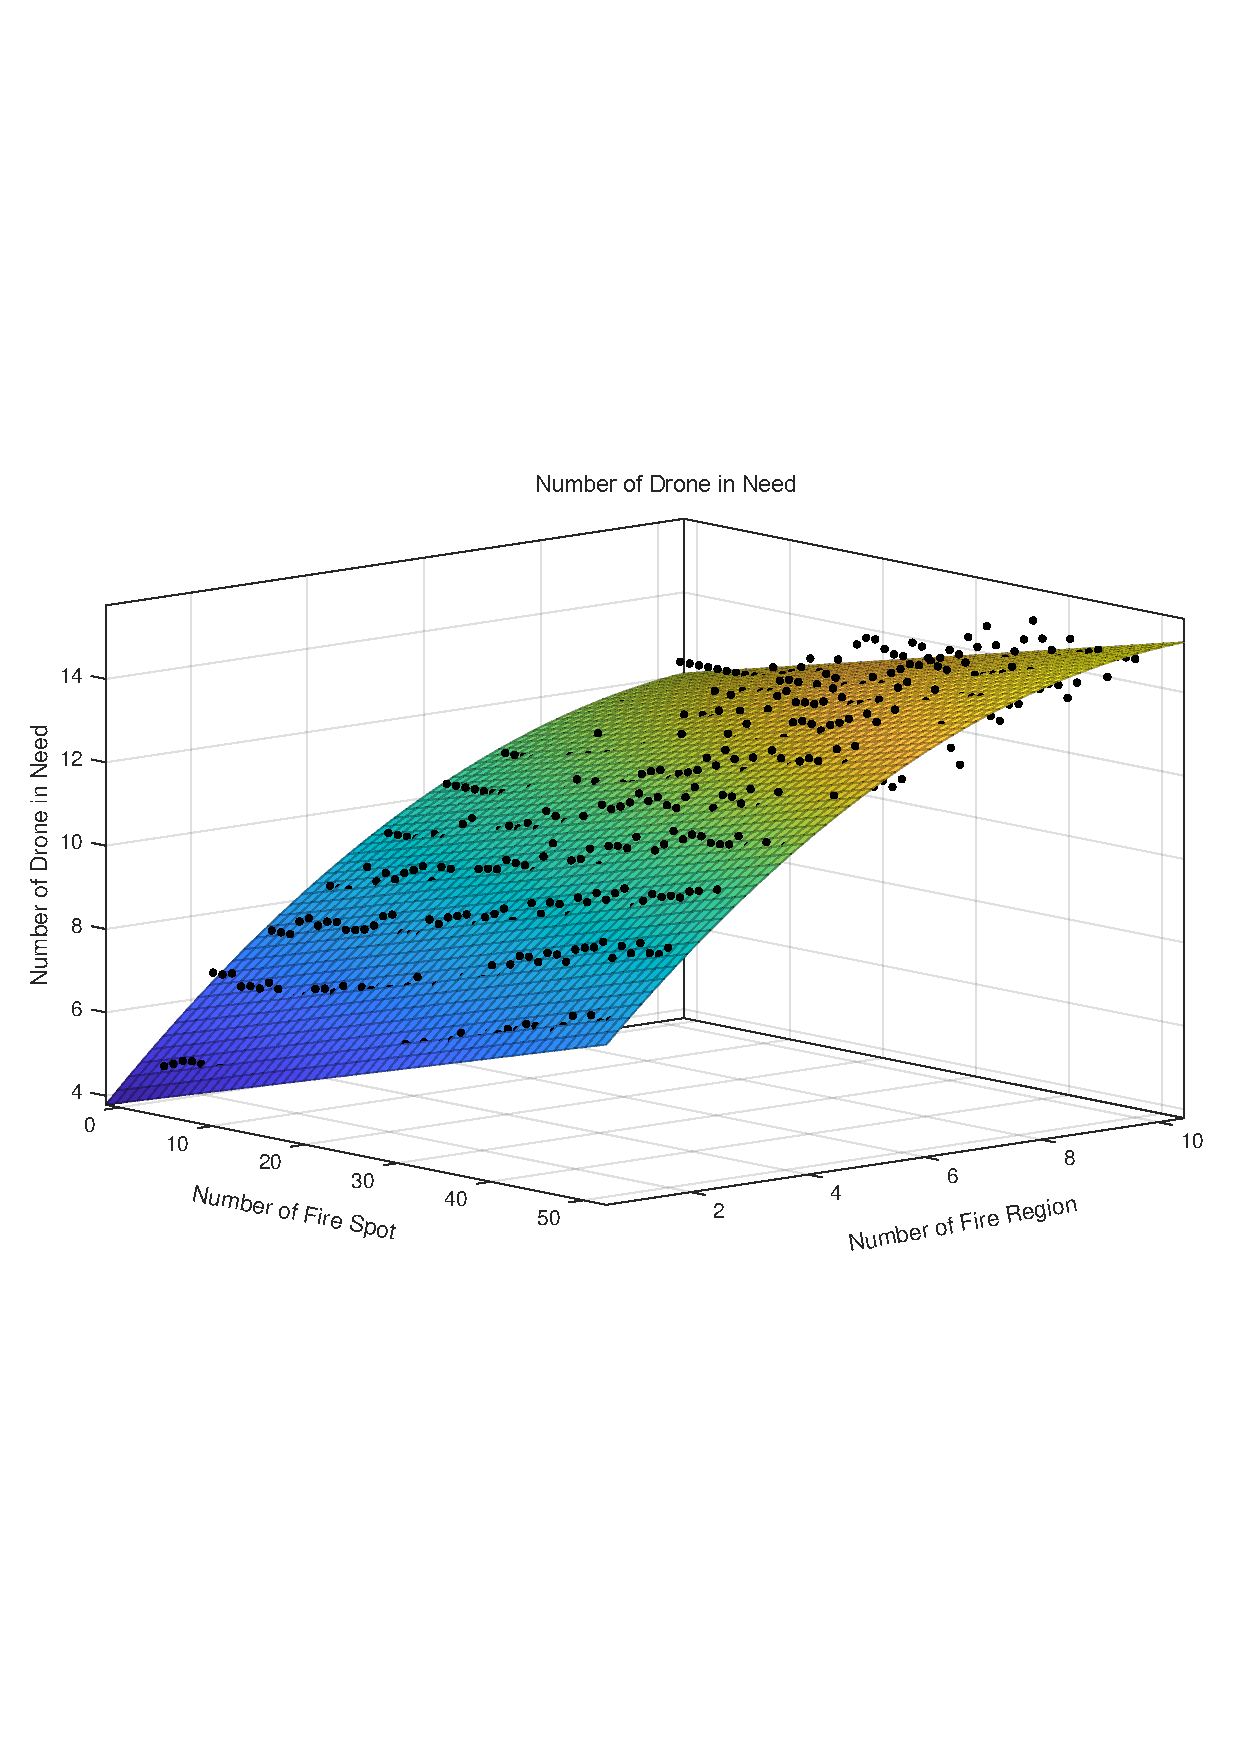
\includegraphics[scale=0.7]{figures/Number_of_Drone_in_Need_fit.pdf}
  \caption{Drone Number Fit}
  \label{Drone Number Fit}
\end{figure}

\begin{figure}[htbp]
  \centering
  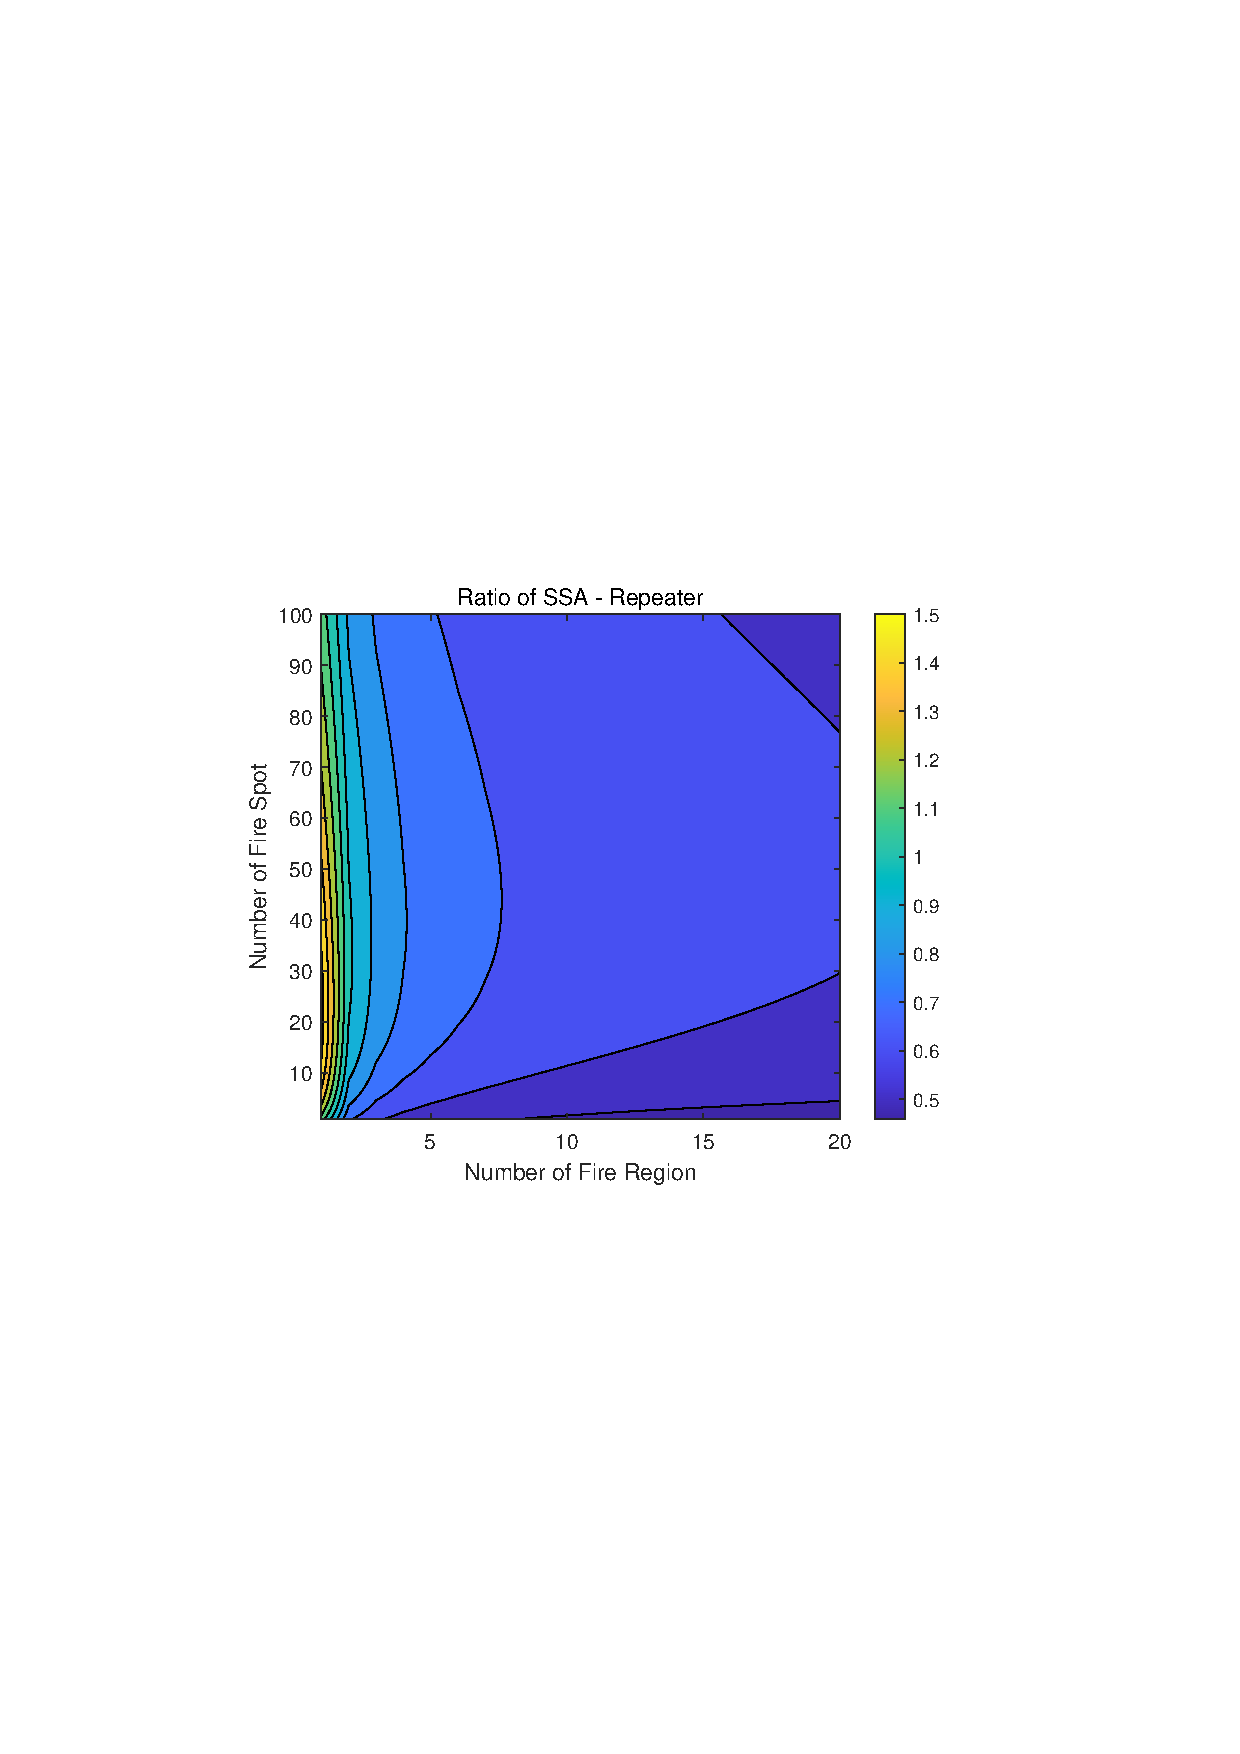
\includegraphics[scale=0.85]{figures/Ratio_of_SSA_Repeater.pdf}
  \caption{Ratio of SSA and RR}
  \label{Ratio of SSA and RR}
\end{figure}

\begin{figure}[htbp]
  \centering
  \includegraphics[scale=0.5]{figures/1.png}
  \caption{Trace of drones}
  \label{Trace}
\end{figure}




%%这里我觉得图片应该补充一些说明,你们解释一下?
\subsection{Results and Anwsers to The Questions}
\subsubsection{For Question 1}

\subsubsection{For Question 2}
\begin{itemize}
  \item \textbf{Normally}, the firespots \textbf{x<10, y<5}, but when encountering
  \textbf{extreme bushfires} \textbf{x=100, y=20}. The increasing of \textbf{x} is far more obvious than \textbf{y}
  \item \textbf{At present}, to respond to normal bushfires, we need 
  $5\times10=50$ drones, with the ratio of RR to SSA is 3:2. But if 
  meets extreme bushfires, $18\times20=360$ drones are required to
  deal with them, with a radio of 2:1 for RR and SSA.
  \item 

\end{itemize}

\subsection{Implemetary}
\textcolor[rgb]{0.98,0.00,0.00}{\textbf{Input C++ source of SSA Counting:}}
\lstinputlisting[language=C++]{./code/SSAnum.cc}


%\section{Sensitivity Analysis}

\section{Disscussion}

\section{Conclusion}
\section{}




\end{document}
%% 
%% This work consists of these files mcmthesis.dtx,
%%                                   figures/ and
%%                                   code/,
%% and the derived files             mcmthesis.cls,
%%                                   mcmthesis-demo.tex,
%%                                   README,
%%                                   LICENSE,
%%                                   mcmthesis.pdf and
%%                                   mcmthesis-demo.pdf.
%%
%% End of file `mcmthesis-demo.tex'.
